% Created by tikzDevice version 0.12.3.1 on 2022-11-04 11:04:43
% !TEX encoding = UTF-8 Unicode
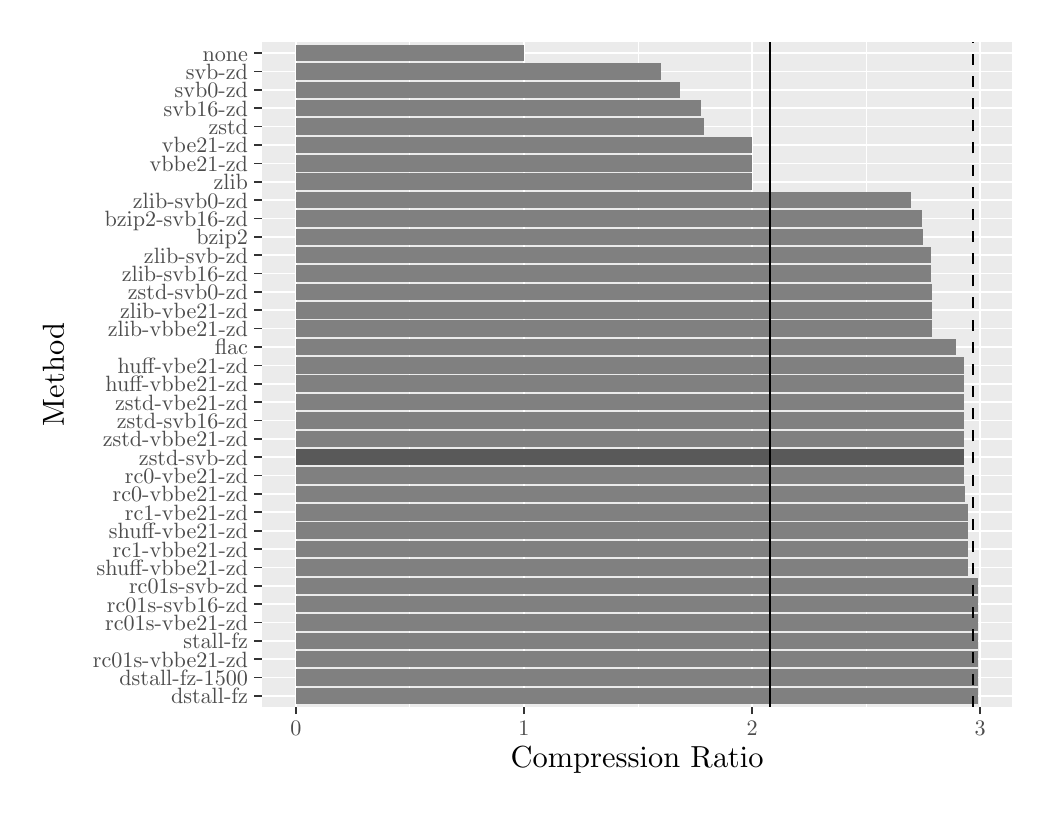
\begin{tikzpicture}[x=1pt,y=0.95pt]
\definecolor{fillColor}{RGB}{255,255,255}
\path[use as bounding box,fill=fillColor,fill opacity=0.00] (0,0) rectangle (361.35,289.08);
\begin{scope}
\path[clip] (  0.00,  0.00) rectangle (361.35,289.08);
\definecolor{drawColor}{RGB}{255,255,255}
\definecolor{fillColor}{RGB}{255,255,255}

\path[draw=drawColor,line width= 0.6pt,line join=round,line cap=round,fill=fillColor] (  0.00,  0.00) rectangle (361.35,289.08);
\end{scope}
\begin{scope}
\path[clip] ( 84.57, 30.69) rectangle (355.85,283.58);
\definecolor{fillColor}{gray}{0.92}

\path[fill=fillColor] ( 84.57, 30.69) rectangle (355.85,283.58);
\definecolor{drawColor}{RGB}{255,255,255}

\path[draw=drawColor,line width= 0.3pt,line join=round] (138.12, 30.69) --
	(138.12,283.58);

\path[draw=drawColor,line width= 0.3pt,line join=round] (220.55, 30.69) --
	(220.55,283.58);

\path[draw=drawColor,line width= 0.3pt,line join=round] (302.98, 30.69) --
	(302.98,283.58);

\path[draw=drawColor,line width= 0.6pt,line join=round] ( 84.57, 34.88) --
	(355.85, 34.88);

\path[draw=drawColor,line width= 0.6pt,line join=round] ( 84.57, 41.86) --
	(355.85, 41.86);

\path[draw=drawColor,line width= 0.6pt,line join=round] ( 84.57, 48.85) --
	(355.85, 48.85);

\path[draw=drawColor,line width= 0.6pt,line join=round] ( 84.57, 55.84) --
	(355.85, 55.84);

\path[draw=drawColor,line width= 0.6pt,line join=round] ( 84.57, 62.82) --
	(355.85, 62.82);

\path[draw=drawColor,line width= 0.6pt,line join=round] ( 84.57, 69.81) --
	(355.85, 69.81);

\path[draw=drawColor,line width= 0.6pt,line join=round] ( 84.57, 76.79) --
	(355.85, 76.79);

\path[draw=drawColor,line width= 0.6pt,line join=round] ( 84.57, 83.78) --
	(355.85, 83.78);

\path[draw=drawColor,line width= 0.6pt,line join=round] ( 84.57, 90.77) --
	(355.85, 90.77);

\path[draw=drawColor,line width= 0.6pt,line join=round] ( 84.57, 97.75) --
	(355.85, 97.75);

\path[draw=drawColor,line width= 0.6pt,line join=round] ( 84.57,104.74) --
	(355.85,104.74);

\path[draw=drawColor,line width= 0.6pt,line join=round] ( 84.57,111.72) --
	(355.85,111.72);

\path[draw=drawColor,line width= 0.6pt,line join=round] ( 84.57,118.71) --
	(355.85,118.71);

\path[draw=drawColor,line width= 0.6pt,line join=round] ( 84.57,125.70) --
	(355.85,125.70);

\path[draw=drawColor,line width= 0.6pt,line join=round] ( 84.57,132.68) --
	(355.85,132.68);

\path[draw=drawColor,line width= 0.6pt,line join=round] ( 84.57,139.67) --
	(355.85,139.67);

\path[draw=drawColor,line width= 0.6pt,line join=round] ( 84.57,146.65) --
	(355.85,146.65);

\path[draw=drawColor,line width= 0.6pt,line join=round] ( 84.57,153.64) --
	(355.85,153.64);

\path[draw=drawColor,line width= 0.6pt,line join=round] ( 84.57,160.63) --
	(355.85,160.63);

\path[draw=drawColor,line width= 0.6pt,line join=round] ( 84.57,167.61) --
	(355.85,167.61);

\path[draw=drawColor,line width= 0.6pt,line join=round] ( 84.57,174.60) --
	(355.85,174.60);

\path[draw=drawColor,line width= 0.6pt,line join=round] ( 84.57,181.58) --
	(355.85,181.58);

\path[draw=drawColor,line width= 0.6pt,line join=round] ( 84.57,188.57) --
	(355.85,188.57);

\path[draw=drawColor,line width= 0.6pt,line join=round] ( 84.57,195.56) --
	(355.85,195.56);

\path[draw=drawColor,line width= 0.6pt,line join=round] ( 84.57,202.54) --
	(355.85,202.54);

\path[draw=drawColor,line width= 0.6pt,line join=round] ( 84.57,209.53) --
	(355.85,209.53);

\path[draw=drawColor,line width= 0.6pt,line join=round] ( 84.57,216.51) --
	(355.85,216.51);

\path[draw=drawColor,line width= 0.6pt,line join=round] ( 84.57,223.50) --
	(355.85,223.50);

\path[draw=drawColor,line width= 0.6pt,line join=round] ( 84.57,230.49) --
	(355.85,230.49);

\path[draw=drawColor,line width= 0.6pt,line join=round] ( 84.57,237.47) --
	(355.85,237.47);

\path[draw=drawColor,line width= 0.6pt,line join=round] ( 84.57,244.46) --
	(355.85,244.46);

\path[draw=drawColor,line width= 0.6pt,line join=round] ( 84.57,251.44) --
	(355.85,251.44);

\path[draw=drawColor,line width= 0.6pt,line join=round] ( 84.57,258.43) --
	(355.85,258.43);

\path[draw=drawColor,line width= 0.6pt,line join=round] ( 84.57,265.42) --
	(355.85,265.42);

\path[draw=drawColor,line width= 0.6pt,line join=round] ( 84.57,272.40) --
	(355.85,272.40);

\path[draw=drawColor,line width= 0.6pt,line join=round] ( 84.57,279.39) --
	(355.85,279.39);

\path[draw=drawColor,line width= 0.6pt,line join=round] ( 96.90, 30.69) --
	( 96.90,283.58);

\path[draw=drawColor,line width= 0.6pt,line join=round] (179.34, 30.69) --
	(179.34,283.58);

\path[draw=drawColor,line width= 0.6pt,line join=round] (261.77, 30.69) --
	(261.77,283.58);

\path[draw=drawColor,line width= 0.6pt,line join=round] (344.20, 30.69) --
	(344.20,283.58);
\definecolor{fillColor}{gray}{0.50}

\path[fill=fillColor] ( 96.90,276.24) rectangle (179.34,282.53);

\path[fill=fillColor] ( 96.90,227.34) rectangle (261.89,233.63);

\path[fill=fillColor] ( 96.90,248.30) rectangle (244.53,254.59);

\path[fill=fillColor] ( 96.90,206.38) rectangle (323.60,212.67);

\path[fill=fillColor] ( 96.90,269.26) rectangle (228.79,275.55);

\path[fill=fillColor] ( 96.90,255.29) rectangle (243.44,261.57);

\path[fill=fillColor] ( 96.90,262.27) rectangle (235.60,268.56);

\path[fill=fillColor] ( 96.90,241.31) rectangle (261.73,247.60);

\path[fill=fillColor] ( 96.90,234.33) rectangle (261.75,240.62);
\definecolor{fillColor}{gray}{0.35}

\path[fill=fillColor] ( 96.90,122.55) rectangle (338.30,128.84);
\definecolor{fillColor}{gray}{0.50}

\path[fill=fillColor] ( 96.90,136.52) rectangle (338.29,142.81);

\path[fill=fillColor] ( 96.90,185.43) rectangle (326.87,191.71);

\path[fill=fillColor] ( 96.90,143.51) rectangle (338.27,149.80);

\path[fill=fillColor] ( 96.90,129.54) rectangle (338.30,135.83);

\path[fill=fillColor] ( 96.90,199.40) rectangle (326.35,205.69);

\path[fill=fillColor] ( 96.90,192.41) rectangle (326.57,198.70);

\path[fill=fillColor] ( 96.90,220.36) rectangle (319.24,226.64);

\path[fill=fillColor] ( 96.90,178.44) rectangle (326.91,184.73);

\path[fill=fillColor] ( 96.90,171.45) rectangle (326.93,177.74);

\path[fill=fillColor] ( 96.90,213.37) rectangle (322.98,219.66);

\path[fill=fillColor] ( 96.90,164.47) rectangle (335.41,170.76);

\path[fill=fillColor] ( 96.90,157.48) rectangle (338.21,163.77);

\path[fill=fillColor] ( 96.90, 94.61) rectangle (339.89,100.90);

\path[fill=fillColor] ( 96.90,115.57) rectangle (338.49,121.85);

\path[fill=fillColor] ( 96.90,101.59) rectangle (339.87,107.88);

\path[fill=fillColor] ( 96.90, 59.68) rectangle (343.45, 65.97);

\path[fill=fillColor] ( 96.90,150.50) rectangle (338.24,156.78);

\path[fill=fillColor] ( 96.90, 80.64) rectangle (339.93, 86.92);

\path[fill=fillColor] ( 96.90,108.58) rectangle (338.52,114.87);

\path[fill=fillColor] ( 96.90, 87.62) rectangle (339.90, 93.91);

\path[fill=fillColor] ( 96.90, 45.71) rectangle (343.48, 51.99);

\path[fill=fillColor] ( 96.90, 52.69) rectangle (343.47, 58.98);

\path[fill=fillColor] ( 96.90, 73.65) rectangle (343.42, 79.94);

\path[fill=fillColor] ( 96.90, 66.66) rectangle (343.42, 72.95);

\path[fill=fillColor] ( 96.90, 31.73) rectangle (343.52, 38.02);

\path[fill=fillColor] ( 96.90, 38.72) rectangle (343.52, 45.01);
\definecolor{drawColor}{RGB}{0,0,0}

\path[draw=drawColor,line width= 0.6pt,line join=round] (268.19, 30.69) -- (268.19,283.58);

\path[draw=drawColor,line width= 0.6pt,dash pattern=on 4pt off 4pt ,line join=round] (341.60, 30.69) -- (341.60,283.58);
\end{scope}
\begin{scope}
\path[clip] (  0.00,  0.00) rectangle (361.35,289.08);
\definecolor{drawColor}{gray}{0.30}

\node[text=drawColor,anchor=base east,inner sep=0pt, outer sep=0pt, scale=  0.80] at ( 79.62, 31.85) {dstall-fz};

\node[text=drawColor,anchor=base east,inner sep=0pt, outer sep=0pt, scale=  0.80] at ( 79.62, 38.83) {dstall-fz-1500};

\node[text=drawColor,anchor=base east,inner sep=0pt, outer sep=0pt, scale=  0.80] at ( 79.62, 45.82) {rc01s-vbbe21-zd};

\node[text=drawColor,anchor=base east,inner sep=0pt, outer sep=0pt, scale=  0.80] at ( 79.62, 52.81) {stall-fz};

\node[text=drawColor,anchor=base east,inner sep=0pt, outer sep=0pt, scale=  0.80] at ( 79.62, 59.79) {rc01s-vbe21-zd};

\node[text=drawColor,anchor=base east,inner sep=0pt, outer sep=0pt, scale=  0.80] at ( 79.62, 66.78) {rc01s-svb16-zd};

\node[text=drawColor,anchor=base east,inner sep=0pt, outer sep=0pt, scale=  0.80] at ( 79.62, 73.76) {rc01s-svb-zd};

\node[text=drawColor,anchor=base east,inner sep=0pt, outer sep=0pt, scale=  0.80] at ( 79.62, 80.75) {shuff-vbbe21-zd};

\node[text=drawColor,anchor=base east,inner sep=0pt, outer sep=0pt, scale=  0.80] at ( 79.62, 87.74) {rc1-vbbe21-zd};

\node[text=drawColor,anchor=base east,inner sep=0pt, outer sep=0pt, scale=  0.80] at ( 79.62, 94.72) {shuff-vbe21-zd};

\node[text=drawColor,anchor=base east,inner sep=0pt, outer sep=0pt, scale=  0.80] at ( 79.62,101.71) {rc1-vbe21-zd};

\node[text=drawColor,anchor=base east,inner sep=0pt, outer sep=0pt, scale=  0.80] at ( 79.62,108.69) {rc0-vbbe21-zd};

\node[text=drawColor,anchor=base east,inner sep=0pt, outer sep=0pt, scale=  0.80] at ( 79.62,115.68) {rc0-vbe21-zd};

\node[text=drawColor,anchor=base east,inner sep=0pt, outer sep=0pt, scale=  0.80] at ( 79.62,122.67) {zstd-svb-zd};

\node[text=drawColor,anchor=base east,inner sep=0pt, outer sep=0pt, scale=  0.80] at ( 79.62,129.65) {zstd-vbbe21-zd};

\node[text=drawColor,anchor=base east,inner sep=0pt, outer sep=0pt, scale=  0.80] at ( 79.62,136.64) {zstd-svb16-zd};

\node[text=drawColor,anchor=base east,inner sep=0pt, outer sep=0pt, scale=  0.80] at ( 79.62,143.62) {zstd-vbe21-zd};

\node[text=drawColor,anchor=base east,inner sep=0pt, outer sep=0pt, scale=  0.80] at ( 79.62,150.61) {huff-vbbe21-zd};

\node[text=drawColor,anchor=base east,inner sep=0pt, outer sep=0pt, scale=  0.80] at ( 79.62,157.60) {huff-vbe21-zd};

\node[text=drawColor,anchor=base east,inner sep=0pt, outer sep=0pt, scale=  0.80] at ( 79.62,164.58) {flac};

\node[text=drawColor,anchor=base east,inner sep=0pt, outer sep=0pt, scale=  0.80] at ( 79.62,171.57) {zlib-vbbe21-zd};

\node[text=drawColor,anchor=base east,inner sep=0pt, outer sep=0pt, scale=  0.80] at ( 79.62,178.55) {zlib-vbe21-zd};

\node[text=drawColor,anchor=base east,inner sep=0pt, outer sep=0pt, scale=  0.80] at ( 79.62,185.54) {zstd-svb0-zd};

\node[text=drawColor,anchor=base east,inner sep=0pt, outer sep=0pt, scale=  0.80] at ( 79.62,192.53) {zlib-svb16-zd};

\node[text=drawColor,anchor=base east,inner sep=0pt, outer sep=0pt, scale=  0.80] at ( 79.62,199.51) {zlib-svb-zd};

\node[text=drawColor,anchor=base east,inner sep=0pt, outer sep=0pt, scale=  0.80] at ( 79.62,206.50) {bzip2};

\node[text=drawColor,anchor=base east,inner sep=0pt, outer sep=0pt, scale=  0.80] at ( 79.62,213.48) {bzip2-svb16-zd};

\node[text=drawColor,anchor=base east,inner sep=0pt, outer sep=0pt, scale=  0.80] at ( 79.62,220.47) {zlib-svb0-zd};

\node[text=drawColor,anchor=base east,inner sep=0pt, outer sep=0pt, scale=  0.80] at ( 79.62,227.46) {zlib};

\node[text=drawColor,anchor=base east,inner sep=0pt, outer sep=0pt, scale=  0.80] at ( 79.62,234.44) {vbbe21-zd};

\node[text=drawColor,anchor=base east,inner sep=0pt, outer sep=0pt, scale=  0.80] at ( 79.62,241.43) {vbe21-zd};

\node[text=drawColor,anchor=base east,inner sep=0pt, outer sep=0pt, scale=  0.80] at ( 79.62,248.41) {zstd};

\node[text=drawColor,anchor=base east,inner sep=0pt, outer sep=0pt, scale=  0.80] at ( 79.62,255.40) {svb16-zd};

\node[text=drawColor,anchor=base east,inner sep=0pt, outer sep=0pt, scale=  0.80] at ( 79.62,262.39) {svb0-zd};

\node[text=drawColor,anchor=base east,inner sep=0pt, outer sep=0pt, scale=  0.80] at ( 79.62,269.37) {svb-zd};

\node[text=drawColor,anchor=base east,inner sep=0pt, outer sep=0pt, scale=  0.80] at ( 79.62,276.36) {none};
\end{scope}
\begin{scope}
\path[clip] (  0.00,  0.00) rectangle (361.35,289.08);
\definecolor{drawColor}{gray}{0.20}

\path[draw=drawColor,line width= 0.6pt,line join=round] ( 81.82, 34.88) --
	( 84.57, 34.88);

\path[draw=drawColor,line width= 0.6pt,line join=round] ( 81.82, 41.86) --
	( 84.57, 41.86);

\path[draw=drawColor,line width= 0.6pt,line join=round] ( 81.82, 48.85) --
	( 84.57, 48.85);

\path[draw=drawColor,line width= 0.6pt,line join=round] ( 81.82, 55.84) --
	( 84.57, 55.84);

\path[draw=drawColor,line width= 0.6pt,line join=round] ( 81.82, 62.82) --
	( 84.57, 62.82);

\path[draw=drawColor,line width= 0.6pt,line join=round] ( 81.82, 69.81) --
	( 84.57, 69.81);

\path[draw=drawColor,line width= 0.6pt,line join=round] ( 81.82, 76.79) --
	( 84.57, 76.79);

\path[draw=drawColor,line width= 0.6pt,line join=round] ( 81.82, 83.78) --
	( 84.57, 83.78);

\path[draw=drawColor,line width= 0.6pt,line join=round] ( 81.82, 90.77) --
	( 84.57, 90.77);

\path[draw=drawColor,line width= 0.6pt,line join=round] ( 81.82, 97.75) --
	( 84.57, 97.75);

\path[draw=drawColor,line width= 0.6pt,line join=round] ( 81.82,104.74) --
	( 84.57,104.74);

\path[draw=drawColor,line width= 0.6pt,line join=round] ( 81.82,111.72) --
	( 84.57,111.72);

\path[draw=drawColor,line width= 0.6pt,line join=round] ( 81.82,118.71) --
	( 84.57,118.71);

\path[draw=drawColor,line width= 0.6pt,line join=round] ( 81.82,125.70) --
	( 84.57,125.70);

\path[draw=drawColor,line width= 0.6pt,line join=round] ( 81.82,132.68) --
	( 84.57,132.68);

\path[draw=drawColor,line width= 0.6pt,line join=round] ( 81.82,139.67) --
	( 84.57,139.67);

\path[draw=drawColor,line width= 0.6pt,line join=round] ( 81.82,146.65) --
	( 84.57,146.65);

\path[draw=drawColor,line width= 0.6pt,line join=round] ( 81.82,153.64) --
	( 84.57,153.64);

\path[draw=drawColor,line width= 0.6pt,line join=round] ( 81.82,160.63) --
	( 84.57,160.63);

\path[draw=drawColor,line width= 0.6pt,line join=round] ( 81.82,167.61) --
	( 84.57,167.61);

\path[draw=drawColor,line width= 0.6pt,line join=round] ( 81.82,174.60) --
	( 84.57,174.60);

\path[draw=drawColor,line width= 0.6pt,line join=round] ( 81.82,181.58) --
	( 84.57,181.58);

\path[draw=drawColor,line width= 0.6pt,line join=round] ( 81.82,188.57) --
	( 84.57,188.57);

\path[draw=drawColor,line width= 0.6pt,line join=round] ( 81.82,195.56) --
	( 84.57,195.56);

\path[draw=drawColor,line width= 0.6pt,line join=round] ( 81.82,202.54) --
	( 84.57,202.54);

\path[draw=drawColor,line width= 0.6pt,line join=round] ( 81.82,209.53) --
	( 84.57,209.53);

\path[draw=drawColor,line width= 0.6pt,line join=round] ( 81.82,216.51) --
	( 84.57,216.51);

\path[draw=drawColor,line width= 0.6pt,line join=round] ( 81.82,223.50) --
	( 84.57,223.50);

\path[draw=drawColor,line width= 0.6pt,line join=round] ( 81.82,230.49) --
	( 84.57,230.49);

\path[draw=drawColor,line width= 0.6pt,line join=round] ( 81.82,237.47) --
	( 84.57,237.47);

\path[draw=drawColor,line width= 0.6pt,line join=round] ( 81.82,244.46) --
	( 84.57,244.46);

\path[draw=drawColor,line width= 0.6pt,line join=round] ( 81.82,251.44) --
	( 84.57,251.44);

\path[draw=drawColor,line width= 0.6pt,line join=round] ( 81.82,258.43) --
	( 84.57,258.43);

\path[draw=drawColor,line width= 0.6pt,line join=round] ( 81.82,265.42) --
	( 84.57,265.42);

\path[draw=drawColor,line width= 0.6pt,line join=round] ( 81.82,272.40) --
	( 84.57,272.40);

\path[draw=drawColor,line width= 0.6pt,line join=round] ( 81.82,279.39) --
	( 84.57,279.39);
\end{scope}
\begin{scope}
\path[clip] (  0.00,  0.00) rectangle (361.35,289.08);
\definecolor{drawColor}{gray}{0.20}

\path[draw=drawColor,line width= 0.6pt,line join=round] ( 96.90, 27.94) --
	( 96.90, 30.69);

\path[draw=drawColor,line width= 0.6pt,line join=round] (179.34, 27.94) --
	(179.34, 30.69);

\path[draw=drawColor,line width= 0.6pt,line join=round] (261.77, 27.94) --
	(261.77, 30.69);

\path[draw=drawColor,line width= 0.6pt,line join=round] (344.20, 27.94) --
	(344.20, 30.69);
\end{scope}
\begin{scope}
\path[clip] (  0.00,  0.00) rectangle (361.35,289.08);
\definecolor{drawColor}{gray}{0.30}

\node[text=drawColor,anchor=base,inner sep=0pt, outer sep=0pt, scale=  0.80] at ( 96.90, 19.68) {0};

\node[text=drawColor,anchor=base,inner sep=0pt, outer sep=0pt, scale=  0.80] at (179.34, 19.68) {1};

\node[text=drawColor,anchor=base,inner sep=0pt, outer sep=0pt, scale=  0.80] at (261.77, 19.68) {2};

\node[text=drawColor,anchor=base,inner sep=0pt, outer sep=0pt, scale=  0.80] at (344.20, 19.68) {3};
\end{scope}
\begin{scope}
\path[clip] (  0.00,  0.00) rectangle (361.35,289.08);
\definecolor{drawColor}{RGB}{0,0,0}

\node[text=drawColor,anchor=base,inner sep=0pt, outer sep=0pt, scale=  1.10] at (220.21,  7.64) {Compression Ratio};
\end{scope}
\begin{scope}
\path[clip] (  0.00,  0.00) rectangle (361.35,289.08);
\definecolor{drawColor}{RGB}{0,0,0}

\node[text=drawColor,rotate= 90.00,anchor=base,inner sep=0pt, outer sep=0pt, scale=  1.10] at ( 13.08,157.13) {Method};
\end{scope}
\end{tikzpicture}
